\documentclass[border=10pt]{standalone}

\usepackage{tikz}
\usepackage{tikzsymbols}
\usetikzlibrary{calc,patterns,shapes.geometric}

\def\centerarc[#1](#2)(#3:#4:#5){\draw[#1] ($(#2)+({#5*cos(#3)},{#5*sin(#3)})$) arc (#3:#4:#5);}

\begin{document}
	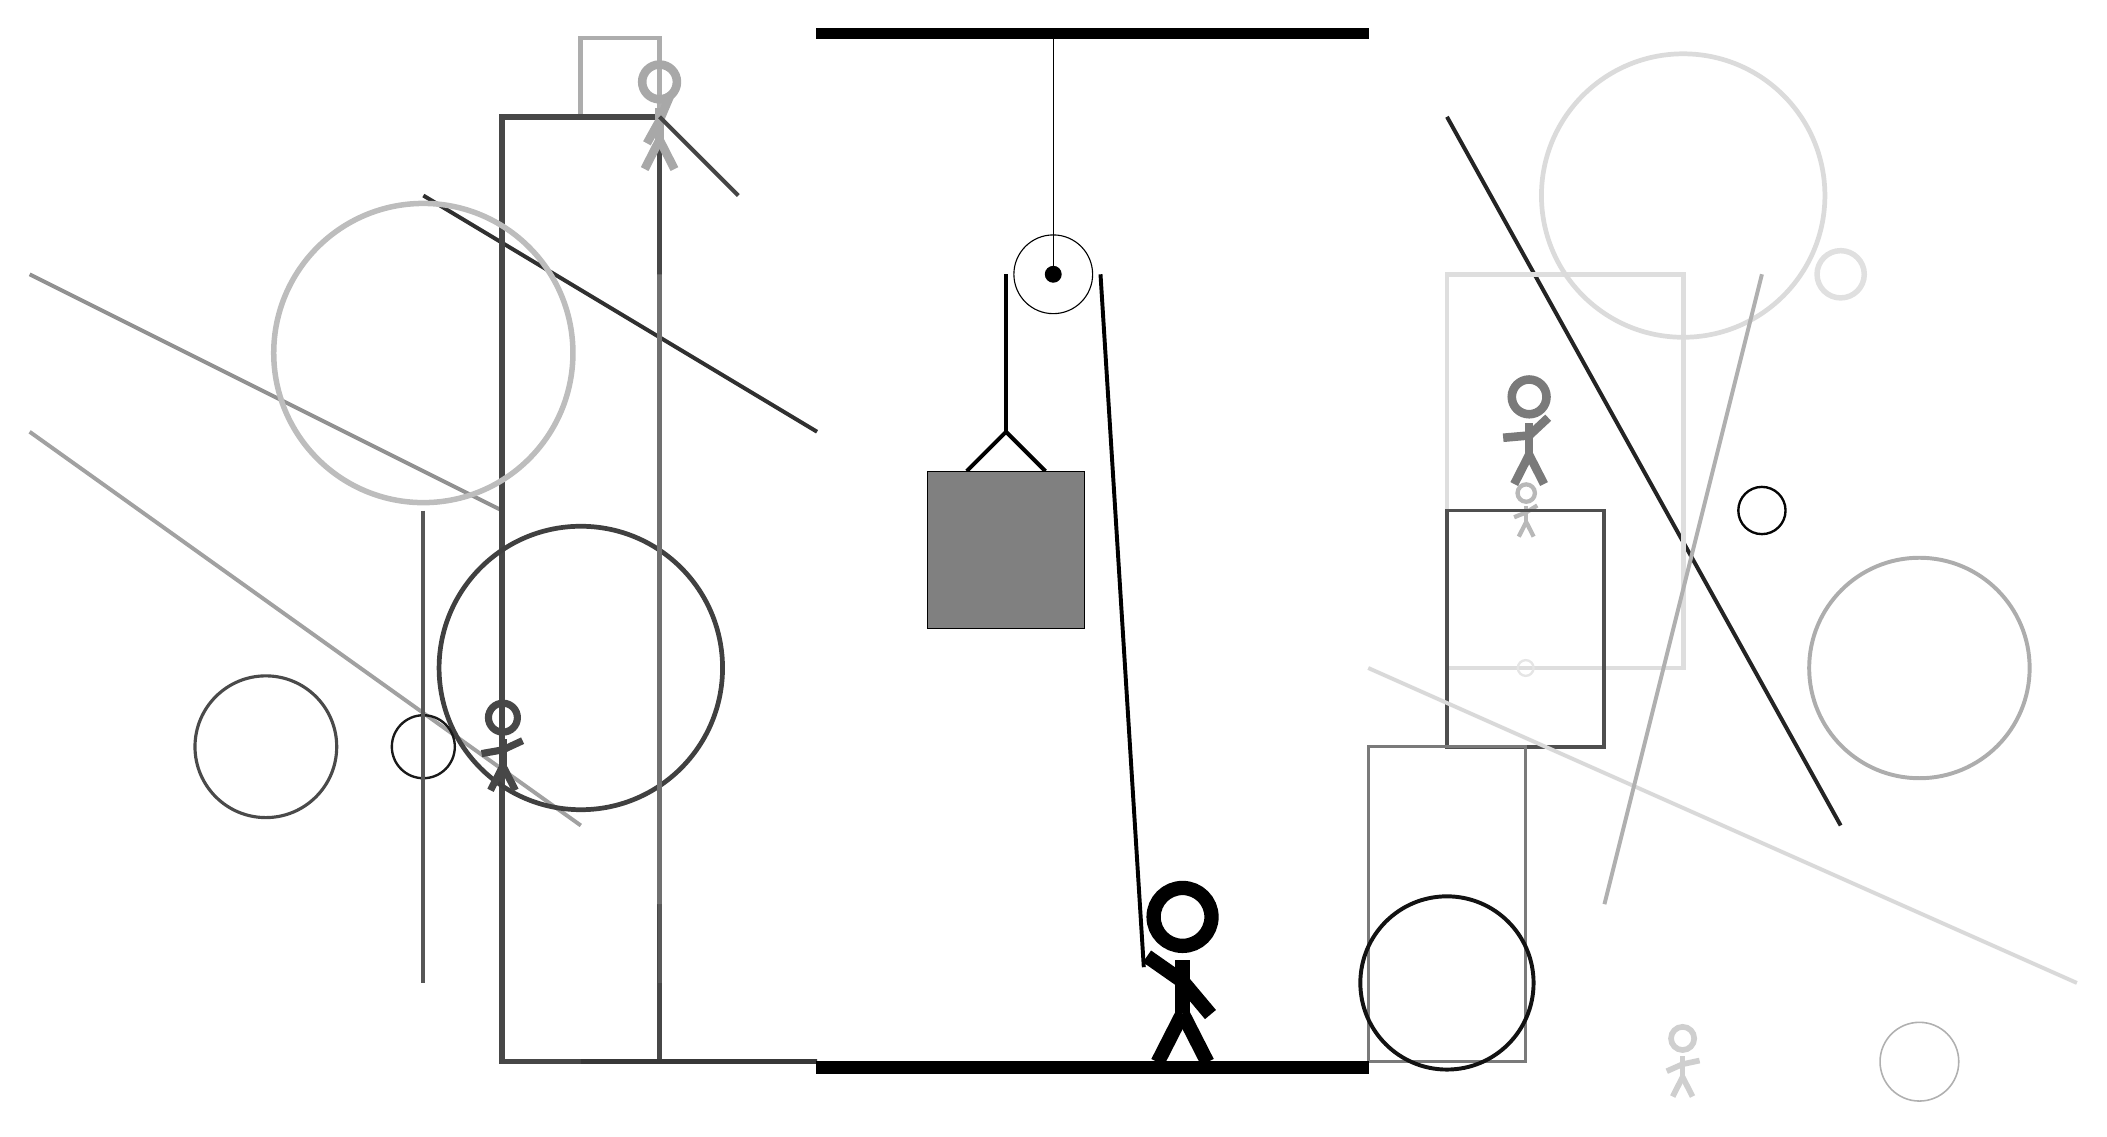
\begin{tikzpicture}
		%%%%% START %%%%%
		
		\draw[fill=black] (-2, 10) rectangle (5, 10.125);
		
		\draw (1, 7) circle (0.5);
		\draw[fill=black] (1, 7) circle (0.1);
		\draw (1, 10) -- (1, 7);
		
		\draw[line width=0.5mm, color=black!81](-7, 8) -- (-2, 5);
		
		\draw [line width=0.2mm, color=black!31](12, -3) circle (0.5);
		\draw[line width=0.6mm, color=black!32] (-4, 9) rectangle (-5, 10);
		\draw[line width=0.5mm, color=black!43](-6, 4) -- (-12, 7);
		\draw [line width=0.7mm, color=black!12](11, 7) circle (0.3);
		\node[line width=0.6mm, color=black!28] at (7, 4) {\Strichmaxerl[3][22][32]};
		\draw[line width=0.7mm, color=black!72] (-4, -3) rectangle (-6, 9);
		\draw[line width=0.5mm, color=black!37](-5, 0) -- (-12, 5);
		\node[line width=0.2mm, color=black!52] at (7, 5) {\Strichmaxerl[6][5][43]};
		\draw [line width=0.6mm, color=black!75](-5, 2) circle (1.8);
		\draw[line width=0.5mm, color=black!86](6, 9) -- (11, 0);
		\draw [line width=0.3mm, color=black!98](10, 4) circle (0.3);
		\draw[line width=0.6mm, color=black!78] (-2, -3) rectangle (-5, -3);
		
		\draw[line width=0.6mm, color=black!13] (6, 2) rectangle (9, 7);
		\draw [line width=0.3mm, color=black!90](-7, 1) circle (0.4);
		\draw [line width=0.7mm, color=black!26](-7, 6) circle (1.9);
		\draw[line width=0.5mm, color=black!69] (6, 4) rectangle (8, 1);
		
		\draw [line width=0.4mm, color=black!71](-9, 1) circle (0.9);
		\draw[line width=0.4mm, color=black!52] (5, 1) rectangle (7, -3);
		
		\draw [line width=0.5mm, color=black!32](12, 2) circle (1.4);
		\draw[line width=0.5mm, color=black!66](-7, 4) -- (-7, -2);
		
		\node[line width=0.3mm, color=black!34] at (-4, 9) {\Strichmaxerl[6][61][67]};
		\node[line width=0.7mm, color=black!72] at (-6, 1) {\Strichmaxerl[5][10][25]};
		\draw[line width=0.5mm, color=black!73](-4, 9) -- (-3, 8);
		\draw [line width=0.5mm, color=black!93](6, -2) circle (1.1);
		
		\node[line width=0.2mm, color=black!19] at (9, -3) {\Strichmaxerl[4][24][12]};
		\draw[line width=0.5mm, color=black!15](5, 2) -- (14, -2);
		\draw [line width=0.3mm, color=black!10](7, 2) circle (0.1);
		
		\draw[line width=0.5mm, color=black!65](-4, 5) -- (-4, -2);
		\draw[line width=0.7mm, color=black!56] (-4, -1) rectangle (-4, 7);
		\draw [line width=0.6mm, color=black!14](9, 8) circle (1.8);
		
		\draw[line width=0.5mm, color=black!31](10, 7) -- (8, -1);
		
		\draw[line width=0.5mm] (-0.1, 4.5) -- (0.4, 5.0) -- (0.9, 4.5);
		\draw[fill=black!50] (-0.6, 4.5) rectangle (1.4, 2.5);
		
		\draw[line width=0.5mm] (0.4, 7) -- (0.4, 5.0);
		\centerarc[line width=0.5mm](1, 7)(0:180:0.6);
		\draw[line width=0.5mm](1.6, 7) -- (2.15, -1.8);
		
		\node at (2.6, -1.9) {\Strichmaxerl[10][-35][-50]};
		
		\draw[fill=black] (-2, -3) rectangle (5, -3.15);
		
		%%%%% END %%%%%
	\end{tikzpicture}
\end{document}